\documentclass[review,3p]{elsarticle}

\usepackage{lineno,hyperref}
\modulolinenumbers[5]
\usepackage{subcaption}             % used in subtable
\usepackage{amsmath,amsfonts,amsthm}            % for subequations

\usepackage{mathtools,amssymb}          % for \leqslant
\newcommand{\ddn}[2]{\frac{\mathrm{d}}{\mathrm{d}#1}#2}
\newcommand{\ddt}{\frac{\mathrm{d}}{\mathrm{d}t}}


\usepackage{upgreek}
\usepackage[dvipsnames]{xcolor}
\usepackage{soul}
\usepackage{multirow}

\usepackage{array}
\newcolumntype{C}[1]{>{\centering\let\newline\\\arraybackslash\hspace{0pt}}m{#1}} 
\newcolumntype{L}[1]{>{\raggedright\let\newline\\\arraybackslash\hspace{0pt}}m{#1}} 
\newcolumntype{R}[1]{>{\raggedleft\let\newline\\\arraybackslash\hspace{0pt}}m{#1}} 

\usepackage{booktabs}       % http://ctan.org/pkg/booktabs

\newcommand{\tabitem}{~~\llap{\textbullet}~~}           % for items inside a table
\usepackage{makecell}       % used inside a table
\usepackage{pbox}           % for weak form 3
\usepackage{empheq}
\newcommand*\widefbox[1]{\fbox{\hspace{2em}#1\hspace{2em}}}


\usepackage{colortbl}
\usepackage{esvect}
\usepackage{spreadtab}
\usepackage{numprint}
\usepackage{xstring}
\renewcommand*{\thefootnote}{\fnsymbol{footnote}}
\usepackage[symbol]{footmisc}

\usepackage{siunitx}

\makeatletter       % for rom in deal.ii symbol
\newcommand*{\rom}[1]{\expandafter\@slowromancap\romannumeral #1@}
\makeatother

\usepackage{enumitem}

\usepackage{cleveref}
\crefformat{section}{\S#2#1#3} % see manual of cleveref, section 8.2.1
\crefformat{subsection}{\S#2#1#3}
\crefformat{subsubsection}{\S#2#1#3}

\captionsetup[figure]{labelfont={bf},name={Fig.},labelsep=period}
\captionsetup[table]{labelfont={bf},name={Table},labelsep=space}

\usepackage[labelformat=simple]{subcaption}	        	% order of subfigure with brackets
\renewcommand\thesubfigure{(\alph{subfigure})}
\renewcommand\thesubtable{(\alph{subtable})}


\usepackage{graphicx}
\usepackage{wrapfig}
\usepackage{lipsum}

\usepackage{pgfplots}       % for tikzpicture

\pdfsuppresswarningpagegroup=1      % eliminate warning 'multiple pdfs with page group included in a single page'

\usepackage[ruled,linesnumbered]{algorithm2e}		% for algorithm


\begin{document}

\section{Numerical results for the benchmark Poisson, diffusion and Helmholtz equations}         \label{discretization_error_bench_pois_diff_Helm}
% 
\subsection{The Poisson equation}         \label{discretization_error_bench_pois}

\subsubsection{$p$ variant}

\begin{figure}[!ht]
    \begin{subfigure}{5.5cm}
        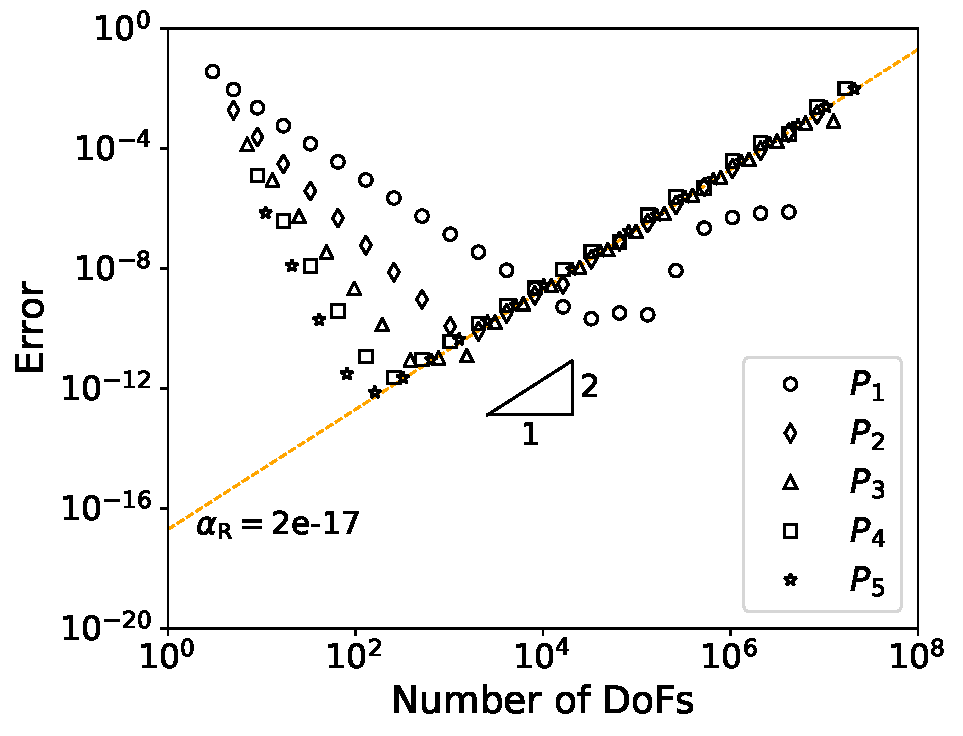
\includegraphics[width=1.0\linewidth]{py_bench_Pois_SM_solu.pdf}			%py_bench_Pois_SM_solu
        \caption{Solution}
        \label{py_bench_Pois_SM_solu}
    \end{subfigure}
    \hspace{-0.2cm}
    \begin{subfigure}{5.5cm}
        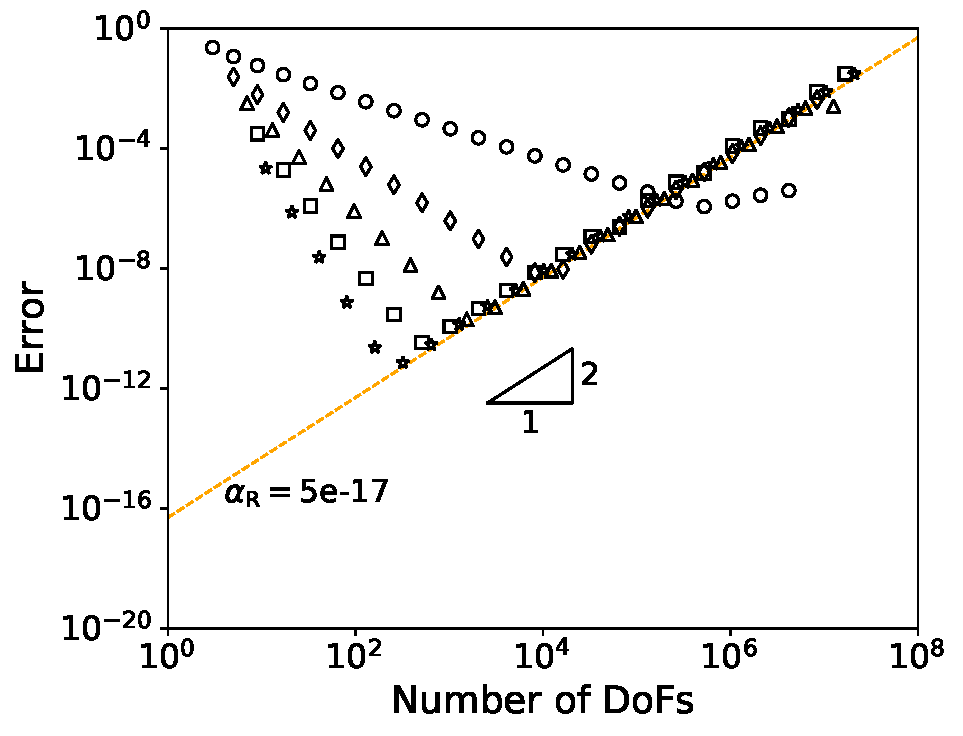
\includegraphics[width=1.0\linewidth]{py_bench_Pois_SM_grad.pdf}
        \caption{First derivative}
        \label{py_bench_Pois_SM_grad}
    \end{subfigure}
    \hspace{-0.2cm}
    \begin{subfigure}{5.5cm}
        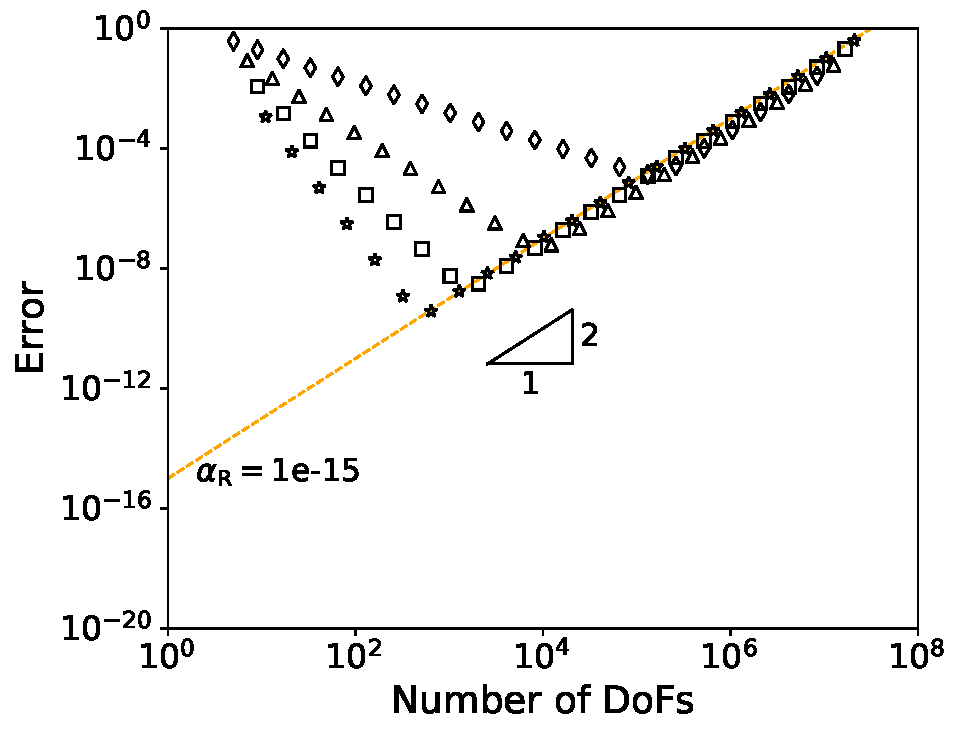
\includegraphics[width=1.0\linewidth]{py_bench_Pois_SM_2ndd.pdf}
        \caption{Second derivative}
        \label{py_bench_Pois_SM_2ndd}
    \end{subfigure}
\caption{Absolute errors for the benchmark Poisson equation using the standard FEM.}
\label{py_bench_Pois_SM}
\end{figure}

\begin{figure}[!ht]
    \begin{subfigure}{5.5cm}
        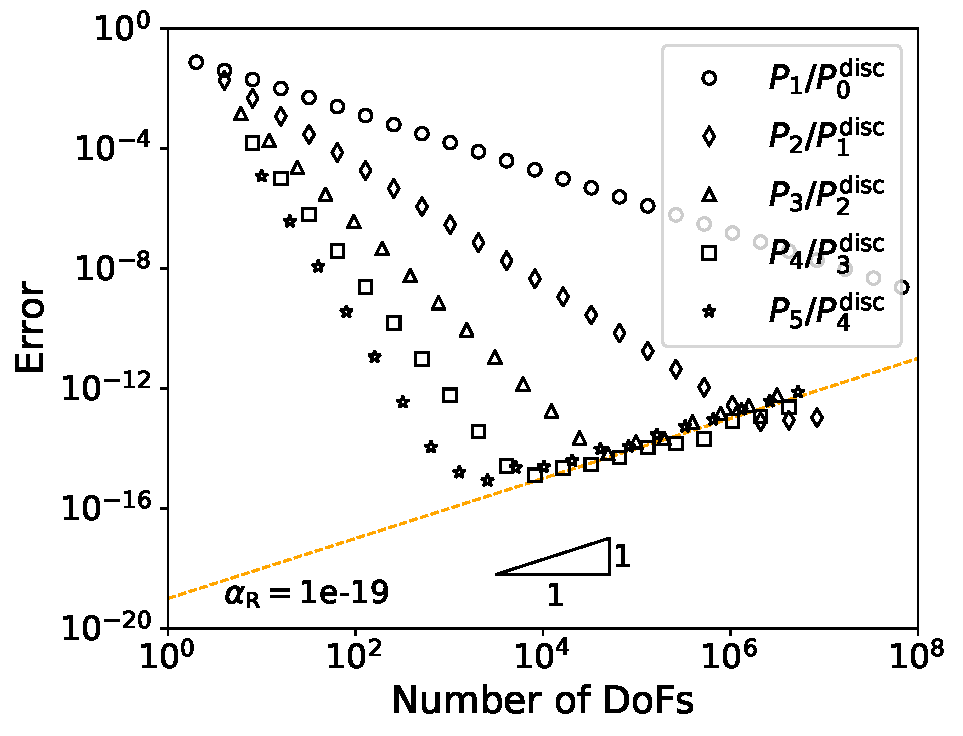
\includegraphics[width=1.0\linewidth]{py_bench_Pois_MM_solu.pdf}
        \caption{Solution}
        \label{py_bench_Pois_MM_solu}
    \end{subfigure}
    \hspace{-0.2cm}
    \begin{subfigure}{5.5cm}
        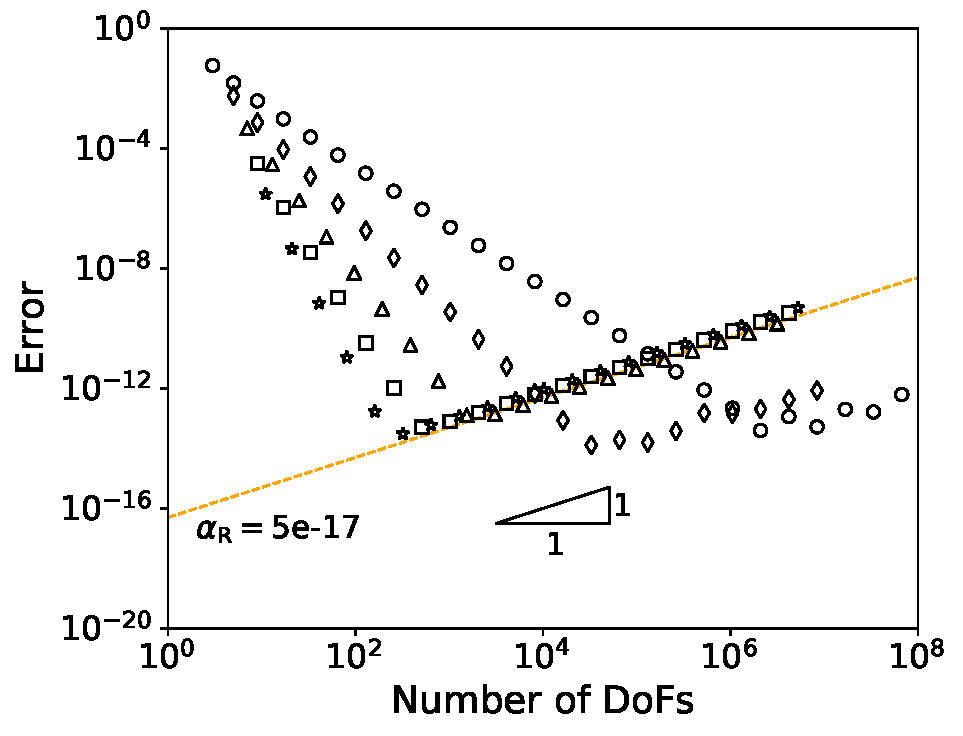
\includegraphics[width=1.0\linewidth]{py_bench_Pois_MM_grad.pdf}
        \caption{First derivative}
        \label{py_bench_Pois_MM_grad}
    \end{subfigure}
    \hspace{-0.2cm}
    \begin{subfigure}{5.5cm}
        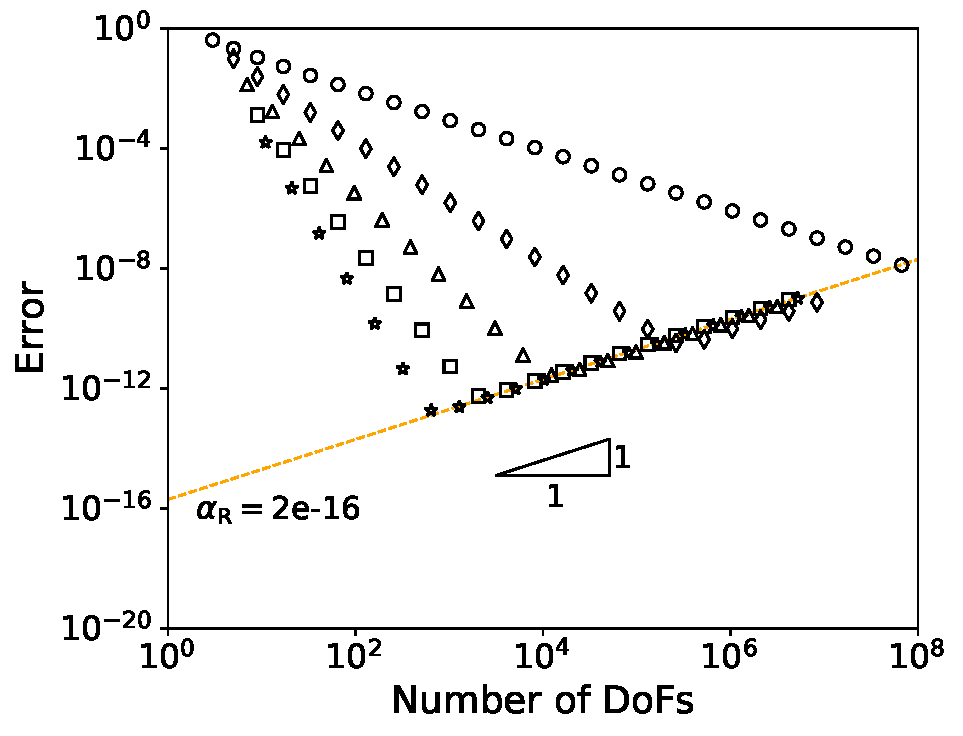
\includegraphics[width=1.0\linewidth]{py_bench_Pois_MM_2ndd.pdf}
        \caption{Second derivative}
        \label{py_bench_Pois_MM_2ndd}
    \end{subfigure}
\caption{Absolute errors for the benchmark Poisson equation using the mixed FEM.}
\label{py_bench_Pois_MM}
\end{figure}

\subsection{\texorpdfstring{The diffusion equation for $p=(2\pi c_1)^{-2}\sin(2\pi c_1x),~d=10$}{The diffusion equation for p=(2pic1){-2}sin(2pic1x), d=10}}

\paragraph{The standard FEM}

\paragraph{The mixed FEM}

\begin{figure}[!ht]
    \begin{subfigure}{5.5cm}
        \includegraphics[width=1.0\linewidth]{py_oned_diff_p_case1_d_10_M0_error_coeff_variant_solu.pdf}
        \caption{Solution}
        \label{py_oned_diff_p_case1_d_10_M0_error_coeff_variant_solu}
    \end{subfigure}
    \hspace{-0.2cm}
    \begin{subfigure}{5.5cm}
        \includegraphics[width=1.0\linewidth]{py_oned_diff_p_case1_d_10_M0_error_coeff_variant_grad.pdf}
        \caption{First derivative}
        \label{py_oned_diff_p_case1_d_10_M0_error_coeff_variant_grad}
    \end{subfigure}
    \hspace{-0.2cm}
    \begin{subfigure}{5.5cm}
        \includegraphics[width=1.0\linewidth]{py_oned_diff_p_case1_d_10_M0_error_coeff_variant_2ndd.pdf}
        \caption{Second derivative}
        \label{py_oned_diff_p_case1_d_10_M0_error_coeff_variant_2ndd}
    \end{subfigure}
\caption{Absolute errors for the diffusion equation with $p=(2\pi c_1)^{-2}\sin(2\pi c_1x),~d=10$ using the mixed FEM, no scaling.}
\label{py_oned_diff_p_case1_d_10_M0_error_coeff_variant}
\end{figure}


% \begin{figure}[!ht]
%     \begin{subfigure}{5.5cm}
%         \includegraphics[width=1.0\linewidth]{py_oned_diff_p_case1_d_10_M1_error_coeff_variant_solu.pdf}
%         \caption{Solution}
%         \label{py_oned_diff_p_case1_d_10_M1_error_coeff_variant_solu}
%     \end{subfigure}
%     \hspace{-0.2cm}
%     \begin{subfigure}{5.5cm}
%         \includegraphics[width=1.0\linewidth]{py_oned_diff_p_case1_d_10_M1_error_coeff_variant_grad.pdf}
%         \caption{First derivative}
%         \label{py_oned_diff_p_case1_d_10_M1_error_coeff_variant_grad}
%     \end{subfigure}
%     \hspace{-0.2cm}
%     \begin{subfigure}{5.5cm}
%         \includegraphics[width=1.0\linewidth]{py_oned_diff_p_case1_d_10_M1_error_coeff_variant_2ndd.pdf}
%         \caption{Second derivative}
%         \label{py_oned_diff_p_case1_d_10_M1_error_coeff_variant_2ndd}
%     \end{subfigure}
% \caption{Absolute errors for the diffusion equation with $p=(2\pi c_1)^{-2}\sin(2\pi c_1x),~d=10$ using the mixed FEM, scheme $M_1$.}
% \label{py_oned_diff_p_case1_d_10_M1_error_coeff_variant}
% \end{figure}

% \begin{figure}[!ht]
%     \begin{subfigure}{5.5cm}
%         \includegraphics[width=1.0\linewidth]{py_oned_diff_p_case1_d_10_M2_error_coeff_variant_solu.pdf}
%         \caption{Solution}
%         \label{py_oned_diff_p_case1_d_10_M2_error_coeff_variant_solu}
%     \end{subfigure}
%     \hspace{-0.2cm}
%     \begin{subfigure}{5.5cm}
%         \includegraphics[width=1.0\linewidth]{py_oned_diff_p_case1_d_10_M2_error_coeff_variant_grad.pdf}
%         \caption{First derivative}
%         \label{py_oned_diff_p_case1_d_10_M2_error_coeff_variant_grad}
%     \end{subfigure}
%     \hspace{-0.2cm}
%     \begin{subfigure}{5.5cm}
%         \includegraphics[width=1.0\linewidth]{py_oned_diff_p_case1_d_10_M2_error_coeff_variant_2ndd.pdf}
%         \caption{Second derivative}
%         \label{py_oned_diff_p_case1_d_10_M2_error_coeff_variant_2ndd}
%     \end{subfigure}
% \caption{Absolute errors for the diffusion equation with $p=(2\pi c_1)^{-2}\sin(2\pi c_1x),~d=10$ using the mixed FEM, scheme $M_2$.}
% \label{py_oned_diff_p_case1_d_10_M2_error_coeff_variant}
% \end{figure}

% \newpage

% When using scheme $M_2$ for $d=1$, $\alpha_{\rm R}$ for $u_x$ is $2\times10^{-17}$. This phenomenon illustrates that $\alpha_{\rm R}$ for $u_x$ depends not only on $\|u\|_2$, but also on $\|d\|_2$.

\newpage

\subsection{\texorpdfstring{The diffusion equation for p=$\sin$(2$\pi$x), d=1+0.5$\sin$(cx)}{The diffusion equation for p=sin(2pix), d=1+0.5sin(cx)}}

To investigate the influence of the oscillation of the diffusion coefficient on the error, we consider $d=1+\frac{1}{2}\sin(cx)$ for the benchmark Poisson equation, resulting the first diffusion equation.
For $c$ ranging from 1 to $10^4$, $\|d\|_2$ is of order 1, see Fig.~\ref{Fig:d_L2_varying_with_c_diff_d_1_plus_sincx}.
The oscillation of $d$ magnifies when $c$ increases.
Using both the standard FEM and the mixed FEM, the errors are shown below.
For the standard FEM, $P_2$ elements are used, and for the mixed FEM, $P_4/P_3^{\rm disc}$ elements are used.

\begin{figure}[!ht]
\centering
    \includegraphics[width=0.45\linewidth]{d_L2_varying_with_c_diff_d_1_plus_sincx.png}
    \caption{Change of $\|d\|_2$ with the coefficient $c$ for the first diffusion equation.}
    \label{Fig:d_L2_varying_with_c_diff_d_1_plus_sincx}   
\end{figure}

\paragraph{The standard FEM}

The truncation error increases when the $d$ oscillates relatively large, i.e. when $c$ is larger than 10.
The lines approximating the round-off error for the solution and first derivative are not affected by the oscillation of $d$, but that for the second derivative moves up a bit when  $c$ is larger than 10.


% the truncation error begins to behave irregularly, i.e. it is larger than the expected value.
% Therefore, for oscillating $d$, irrespective of $\|d\|_2$, the error would be affected.


\begin{figure}[!ht]
    \begin{subfigure}{5.5cm}
        \includegraphics[width=1.0\linewidth]{py_oned_diff_p_exp_minus_x_minus_0p5_square_SM_error_normal_coeff_variant_solu.pdf}
        \caption{Solution}
        \label{py_oned_diff_p_exp_minus_x_minus_0p5_square_SM_error_normal_coeff_variant_solu}
    \end{subfigure}
    \hspace{-0.2cm}
    \begin{subfigure}{5.5cm}
        \includegraphics[width=1.0\linewidth]{py_oned_diff_p_exp_minus_x_minus_0p5_square_SM_error_normal_coeff_variant_grad.pdf}
        \caption{First derivative}
        \label{py_oned_diff_p_exp_minus_x_minus_0p5_square_SM_error_normal_coeff_variant_grad}
    \end{subfigure}
    \hspace{-0.2cm}
    \begin{subfigure}{5.5cm}
        \includegraphics[width=1.0\linewidth]{py_oned_diff_p_exp_minus_x_minus_0p5_square_SM_error_normal_coeff_variant_2ndd.pdf}
        \caption{Second derivative}
        \label{py_oned_diff_p_exp_minus_x_minus_0p5_square_SM_error_normal_coeff_variant_2ndd}
    \end{subfigure}
\caption{Absolute errors for the first diffusion equation using the standard FEM.}
\label{py_oned_diff_p_exp_minus_x_minus_0p5_square_SM_error_normal_coeff_variant}
\end{figure}

\newpage
\paragraph{The mixed FEM}

The truncation error increases when $d$ oscillates relatively large.
% For the solution, 
The lines approximating the round-off error are not affected.


\begin{figure}[!ht]
    \begin{subfigure}{5.5cm}
        \includegraphics[width=1.0\linewidth]{py_oned_bench_diff_p_exp_minus_x_minus_0p5_square_MM_normal_error_coeff_variant_solu.pdf}
        \caption{Solution}
        \label{py_oned_bench_diff_p_exp_minus_x_minus_0p5_square_MM_normal_error_coeff_variant_solu}
    \end{subfigure}
    \hspace{-0.2cm}
    \begin{subfigure}{5.5cm}
        \includegraphics[width=1.0\linewidth]{py_oned_bench_diff_p_exp_minus_x_minus_0p5_square_MM_normal_error_coeff_variant_grad.pdf}
        \caption{First derivative}
        \label{py_oned_bench_diff_p_exp_minus_x_minus_0p5_square_MM_normal_error_coeff_variant_grad}
    \end{subfigure}
    \hspace{-0.2cm}
    \begin{subfigure}{5.5cm}
        \includegraphics[width=1.0\linewidth]{py_oned_bench_diff_p_exp_minus_x_minus_0p5_square_MM_normal_error_coeff_variant_2ndd.pdf}
        \caption{Second derivative}
        \label{py_oned_bench_diff_p_exp_minus_x_minus_0p5_square_MM_normal_error_coeff_variant_2ndd}
    \end{subfigure}
\caption{Absolute errors for the first diffusion equation using the mixed FEM.}
\label{py_oned_bench_diff_p_exp_minus_x_minus_0p5_square_MM_normal_error_coeff_variant}
\end{figure}

Last but not least, the offsets $\alpha_{\rm R}$ tend to be smaller than that of the Poisson equation.

% 
\newpage
\subsection{\texorpdfstring{The diffusion equation for p=$\sin$(2$\pi$x), d=1+cx}{The diffusion equation for p=sin(2pix), d=1+cx}} \label{discretization_error_bench_diff}

We consider the diffusion equation shown in Table 1 in \cite{liu2019balancing}.
We first find the offsets $\alpha_{\rm R}$ for the diffusion equation using recommended scaling schemes for the standard and mixed FEMs, in which the element degree $p$ ranges from 1 to 5.
Next, we investigate $\alpha_{\rm R}$ for different coefficients, i.e. $d(x)=1+cx$ with $c$ ranging from $10^{-4}$ to $10^4$, in which $P_2$ elements are used for the standard FEM, and $P_4/P_3^{\rm disc}$ elements are used for the mixed FEM.

\subsubsection{$p$ variant}

\paragraph{The standard FEM}

Not using scaling and using scheme $S$, the errors are shown in Fig.~\ref{py_oned_bench_diff_SM_error_p_variant}. 

\begin{figure}[!ht]
    \begin{subfigure}{5.5cm}
        \includegraphics[width=1.0\linewidth]{py_oned_bench_diff_SM_error_p_variant_solu.pdf}
        \caption{Solution}
        \label{py_oned_bench_diff_SM_error_p_variant_solu}
    \end{subfigure}
    \hspace{-0.2cm}
    \begin{subfigure}{5.5cm}
        \includegraphics[width=1.0\linewidth]{py_oned_bench_diff_SM_error_p_variant_grad.pdf}
        \caption{First derivative}
        \label{py_oned_bench_diff_SM_error_p_variant_grad}
    \end{subfigure}
    \hspace{-0.2cm}
    \begin{subfigure}{5.5cm}
        \includegraphics[width=1.0\linewidth]{py_oned_bench_diff_SM_error_p_variant_2ndd.pdf}
        \caption{Second derivative}
        \label{py_oned_bench_diff_SM_error_p_variant_2ndd}
    \end{subfigure}
\caption{Absolute errors for the benchmark diffusion equation using the standard FEM. The black color denotes results without scaling, and the green color denotes results using scheme $S$.}
\label{py_oned_bench_diff_SM_error_p_variant}
\end{figure}


% \newpage
\paragraph{The mixed FEM}
Not using scaling and using schemes $M_1$ and $M_2$, the errors are shown in Fig.~\ref{py_oned_bench_diff_MM_error_p_variant_all}. 

\begin{figure}[!ht]
    \begin{subfigure}{5.4cm}
        \includegraphics[width=1.0\linewidth]{py_oned_bench_diff_MM_error_p_variant_all_solu.pdf}
        \caption{Solution}
        \label{py_oned_bench_diff_MM_error_p_variant_all_solu}
    \end{subfigure}
    \hspace{-0.18cm}
    \begin{subfigure}{5.4cm}
        \includegraphics[width=1.0\linewidth]{py_oned_bench_diff_MM_error_p_variant_all_grad.pdf}
        \caption{First derivative}
        \label{py_oned_bench_diff_MM_error_p_variant_all_grad}
    \end{subfigure}
    \hspace{-0.18cm}
    \begin{subfigure}{5.4cm}
        \includegraphics[width=1.0\linewidth]{py_oned_bench_diff_MM_error_p_variant_all_2ndd.pdf}
        \caption{Second derivative}
        \label{py_oned_bench_diff_MM_error_p_variant_all_2ndd}
    \end{subfigure}
\caption{Absolute errors for the benchmark diffusion equation using the mixed FEM. The black color denotes results without scaling, the green color denotes results using scheme $M_1$ and the violet color denotes results using scheme $M_2$. }
\label{py_oned_bench_diff_MM_error_p_variant_all}    
\end{figure}
\newpage

The offsets $\alpha_{\rm R}$ for different scaling schemes are summarized in Fig.~\ref{alpha_R_diff}.
For the standard FEM, $\alpha_{\rm R}$ are basically the same using scheme $S$ or not.
For the mixed FEM, $\alpha_{\rm R}$ changes a bit for different scaling schemes.

\begin{figure}[!ht]
\hspace{2.2cm}
% \centering
\begin{subfigure}[b]{0.4\textwidth}
\scalebox{0.9}{
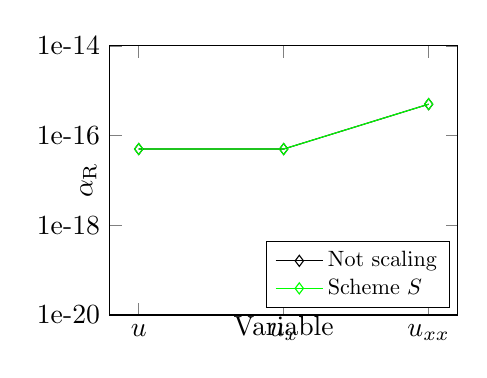
\begin{tikzpicture} 
\begin{axis}
[
    ymode=log,    
    ymin=1e-20,
    ymax=1e-14,
    ytick={1e-20, 1e-18, 1e-16, 1e-14},
    yticklabels={1e-20, 1e-18, 1e-16, 1e-14},        
    legend style={nodes={scale=0.8},at={(0.45,0.15)},anchor=west},
    legend cell align={left},
    height=5cm,
    width=6cm,
    ylabel={$\alpha_{\rm R}$},
    ylabel style={at={(-0.01,0.5)}},    
    xtick={0,1,2,3,4},
    xticklabels={$u$,$u_x$, $u_{xx}$, $4$, ${5}$},
    xlabel={Variable},
    xlabel style={at={(0.5,0.03)}},    
]
\addplot[black,mark=diamond,mark options={color=black,fill=black}] coordinates {(0,5.0e-17) (1,5.0e-17) (2,5.0e-16)};
\addplot[green,mark=diamond,mark options={color=green,fill=green}] coordinates {(0,5.0e-17) (1,5.0e-17) (2,5.0e-16)};
\legend{Not scaling, Scheme $S$};
\end{axis}
\end{tikzpicture}
}
\caption{The standard FEM}
\label{alpha_R_diff_std}
\end{subfigure}
\hspace{-1.0cm}
\begin{subfigure}[b]{0.4\textwidth}
\scalebox{0.9}{
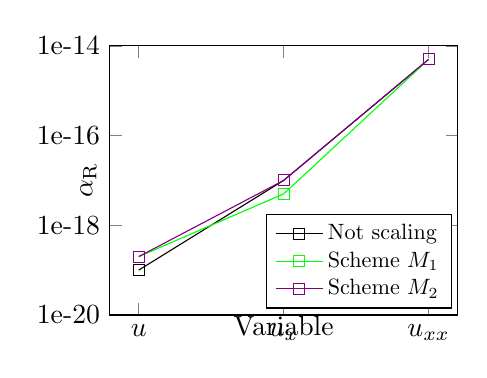
\begin{tikzpicture} 
\begin{axis}
[
    ymode=log,    
    ymin=1e-20,
    ymax=1e-14,
    ytick={1e-20, 1e-18, 1e-16, 1e-14},
    yticklabels={1e-20, 1e-18, 1e-16, 1e-14},        
    legend style={nodes={scale=0.8},at={(0.45,0.2)},anchor=west},
    legend cell align={left},
    height=5cm,
    width=6cm,
    ylabel={$\alpha_{\rm R}$},
    ylabel style={at={(-0.01,0.5)}},    
    xtick={0,1,2,3,4},
    xticklabels={$u$,$u_x$, $u_{xx}$, $4$, ${5}$},
    xlabel={Variable},
    xlabel style={at={(0.5,0.03)}},    
]
\addplot[black,mark=square,mark options={color=black,fill=black}] coordinates {(0, 1.0e-19) (1, 1.0e-17) (2, 5.0e-15)};
\addplot[green,mark=square,mark options={color=green,fill=green}] coordinates {(0, 2.0e-19) (1, 5.0e-18) (2, 5.0e-15)};
\addplot[violet,mark=square,mark options={color=violet,fill=violet}] coordinates {(0, 2.0e-19) (1, 1.0e-17) (2, 5.0e-15)};
\legend{Not scaling, Scheme $M_1$, Scheme $M_2$};
\end{axis}
\end{tikzpicture}
}
\caption{The mixed FEM}
\label{alpha_R_diff_mix}
\end{subfigure}
\caption{$\alpha_{\rm R}$ for the benchmark diffusion equation for different scaling schemes.}
\label{alpha_R_diff}
\end{figure}

\subsubsection{$c$ variant}

The values of $\|d\|_2$ for different $c$ are given in Fig.~\ref{Fig:d_L2_varying_with_c_diff}.
It shows that when $c<1$, $\|d\|_2$ are basically the same; when $c>1$, $\|d\|_2$ increases quickly.

\begin{figure}[!ht]
\centering
    \includegraphics[width=0.45\linewidth]{d_L2_varying_with_c_diff.png}
    \caption{Change of $\|d\|_2$ with the coefficient $c$ for the diffusion equation.}
    \label{Fig:d_L2_varying_with_c_diff}   
\end{figure}

\newpage
\paragraph{The standard FEM}

Using scheme $S$, the errors are shown in Fig.~\ref{py_oned_bench_diff_SM_error_scheme_S_coeff_variant}.
When $c<1$, like $\|d\|_2$, $\alpha_{\rm R}$ for different $c$ are basically the same; when $c>1$, $\alpha_{\rm R}$ increases with $c$, and the magnitude of the increase is larger for higher-order derivatives.

\begin{figure}[!ht]
    \begin{subfigure}{5.5cm}
        \includegraphics[width=1.0\linewidth]{py_oned_bench_diff_SM_error_scheme_S_coeff_variant_solu.pdf}
        \caption{Solution}
        \label{py_oned_bench_diff_SM_error_scheme_S_coeff_variant_solu}
    \end{subfigure}
    \hspace{-0.2cm}
    \begin{subfigure}{5.5cm}
        \includegraphics[width=1.0\linewidth]{py_oned_bench_diff_SM_error_scheme_S_coeff_variant_grad.pdf}
        \caption{First derivative}
        \label{py_oned_bench_diff_SM_error_scheme_S_coeff_variant_grad}
    \end{subfigure}
    \hspace{-0.2cm}
    \begin{subfigure}{5.5cm}
        \includegraphics[width=1.0\linewidth]{py_oned_bench_diff_SM_error_scheme_S_coeff_variant_2ndd.pdf}
        \caption{Second derivative}
        \label{py_oned_bench_diff_SM_error_scheme_S_coeff_variant_2ndd}
    \end{subfigure}
\caption{Absolute errors for the benchmark diffusion equation using the standard FEM with scheme $S$, $c$ variant.}
\label{py_oned_bench_diff_SM_error_scheme_S_coeff_variant}
\end{figure}

\begin{figure}[!ht]
    \begin{subfigure}{5.5cm}
        \includegraphics[width=1.0\linewidth]{py_error_oned_diff_p_sin2pix_d_1pcx_S1_c_var_solu.pdf}
        \caption{Solution}
        \label{py_error_oned_diff_p_sin2pix_d_1pcx_S1_c_var_solu}
    \end{subfigure}
    \hspace{-0.2cm}
    \begin{subfigure}{5.5cm}
        \includegraphics[width=1.0\linewidth]{py_error_oned_diff_p_sin2pix_d_1pcx_S1_c_var_grad.pdf}
        \caption{First derivative}
        \label{py_error_oned_diff_p_sin2pix_d_1pcx_S1_c_var_grad}
    \end{subfigure}
    \hspace{-0.2cm}
    \begin{subfigure}{5.5cm}
        \includegraphics[width=1.0\linewidth]{py_error_oned_diff_p_sin2pix_d_1pcx_S1_c_var_2ndd.pdf}
        \caption{Second derivative}
        \label{py_error_oned_diff_p_sin2pix_d_1pcx_S1_c_var_2ndd}
    \end{subfigure}
\caption{Absolute errors for the benchmark diffusion equation but only imposed by Dirichlet boundary conditions using the standard FEM with scheme $S$, $c$ variant.}
\label{py_error_oned_diff_p_sin2pix_d_1pcx_S1_c_var}
\end{figure}

To clarify if the increase of $\alpha_{\rm R}$ for higher-order derivatives is caused by the magnitude of $\|d\|_2$, we divide the equation by $\|d\|_2$, which results in
\begin{equation}
 -(d/{\|d\|_2} u_x)_x = f/{\|d\|_2}.             \label{diff_eq_coeff_scaling}
\end{equation}

For the above equation, the errors of the solution, first and second derivatives are shown in Fig.~\ref{py_oned_bench_diff_SM_error_scheme_S_diff_coeff_variant}. It shows that $\alpha_{\rm R}$ also increases when $c$ is relatively large.


\begin{figure}[!ht]
    \begin{subfigure}{5.5cm}
        \includegraphics[width=1.0\linewidth]{py_oned_bench_diff_SM_error_scheme_S_diff_coeff_variant_solu.pdf}
        \caption{Solution}
        \label{py_oned_bench_diff_SM_error_scheme_S_diff_coeff_variant_solu}
    \end{subfigure}
    \hspace{-0.2cm}
    \begin{subfigure}{5.5cm}
        \includegraphics[width=1.0\linewidth]{py_oned_bench_diff_SM_error_scheme_S_diff_coeff_variant_grad.pdf}
        \caption{First derivative}
        \label{py_oned_bench_diff_SM_error_scheme_S_diff_coeff_variant_grad}
    \end{subfigure}
    \hspace{-0.2cm}
    \begin{subfigure}{5.5cm}
        \includegraphics[width=1.0\linewidth]{py_oned_bench_diff_SM_error_scheme_S_diff_coeff_variant_2ndd.pdf}
        \caption{Second derivative}
        \label{py_oned_bench_diff_SM_error_scheme_S_diff_coeff_variant_2ndd}
    \end{subfigure}
\caption{Absolute errors for Eq.~(\ref{diff_eq_coeff_scaling}) using the standard FEM, no scaling, $c$ variant.}
\label{py_oned_bench_diff_SM_error_scheme_S_diff_coeff_variant}
\end{figure}

\newpage
\paragraph{The mixed FEM}
Not using scaling, the errors are shown in Fig.~\ref{py_oned_bench_diff_M0_error_coeff_variant_nonpost}.
It shows that when $c$ is relatively large, $\alpha_{\rm R}$ for the first and second derivatives increases. This is because the magnitude of the first derivative, which is $\|du_x\|_2$, increases with $c$ when $c>1$.

\begin{figure}[!ht]
    \begin{subfigure}{5.5cm}
        \includegraphics[width=1.0\linewidth]{py_oned_bench_diff_M0_error_coeff_variant_nonpost_solu.pdf}
        \caption{Solution}
        \label{py_oned_bench_diff_M0_error_coeff_variant_nonpost_solu}
    \end{subfigure}
    \hspace{-0.2cm}
    \begin{subfigure}{5.5cm}
        \includegraphics[width=1.0\linewidth]{py_oned_bench_diff_M0_error_coeff_variant_nonpost_grad.pdf}
        \caption{First derivative}
        \label{py_oned_bench_diff_M0_error_coeff_variant_nonpost_grad}
    \end{subfigure}
    \hspace{-0.2cm}
    \begin{subfigure}{5.5cm}
        \includegraphics[width=1.0\linewidth]{py_oned_bench_diff_M0_error_coeff_variant_nonpost_2ndd.pdf}
        \caption{Second derivative}
        \label{py_oned_bench_diff_M0_error_coeff_variant_nonpost_2ndd}
    \end{subfigure}
\caption{Absolute errors for the benchmark diffusion equation using the mixed FEM with $P_4/P_3^{\rm disc}$ elements, $v=-du_x$, coefficient variant, no scaling.}
\label{py_oned_bench_diff_M0_error_coeff_variant_nonpost}
\end{figure}

% \newpage

If we use scheme $M_1$ in \cite{liu2019balancing}, the errors are shown in Fig.~\ref{py_oned_bench_diff_M1_error_coeff_variant_nonpost}, where the convergence behavior of $\alpha_{\rm R}$ is observed. Note that, $\|v\|_2$ is $\|du_x\|_2$ for the diffusion equation.

\begin{figure}[!ht]
    \begin{subfigure}{5.5cm}
        \includegraphics[width=1.0\linewidth]{py_oned_bench_diff_M1_error_coeff_variant_nonpost_solu.pdf}
        \caption{Solution}
        \label{py_oned_bench_diff_M1_error_coeff_variant_nonpost_solu}
    \end{subfigure}
    \hspace{-0.2cm}
    \begin{subfigure}{5.5cm}
        \includegraphics[width=1.0\linewidth]{py_oned_bench_diff_M1_error_coeff_variant_nonpost_grad.pdf}
        \caption{First derivative}
        \label{py_oned_bench_diff_M1_error_coeff_variant_nonpost_grad}
    \end{subfigure}
    \hspace{-0.2cm}
    \begin{subfigure}{5.5cm}
        \includegraphics[width=1.0\linewidth]{py_oned_bench_diff_M1_error_coeff_variant_nonpost_2ndd.pdf}
        \caption{Second derivative}
        \label{py_oned_bench_diff_M1_error_coeff_variant_nonpost_2ndd}
    \end{subfigure}
\caption{Absolute errors for the benchmark diffusion equation using the mixed FEM with $P_4/P_3^{\rm disc}$ elements, $v=-du_x$, coefficient variant, scheme $M_1$.}
\label{py_oned_bench_diff_M1_error_coeff_variant_nonpost}
\end{figure}


\newpage

\subsection{The Helmholtz equation}

For $d(x)=1+0.5 \sin(x)$, we consider the influence of the magnitude of $r(x)$ on the error.
We consider $r(x)$ as a constant, which ranges from 1 to $10^8$.

\paragraph{The standard FEM}
We use $P_2$ elements. The errors are shown in Fig.~\ref{py_oned_helm_p_exp_minus_x_minus_0p5_square_d_1_plus_0p5sinx_SM_error_normal_coeff_variant}.

\begin{figure}[!ht]
    \begin{subfigure}{5.5cm}
        \includegraphics[width=1.0\linewidth]{py_oned_helm_p_exp_minus_x_minus_0p5_square_d_1_plus_0p5sinx_SM_error_normal_coeff_variant_solu.pdf}
        \caption{Solution}
        \label{py_oned_helm_p_exp_minus_x_minus_0p5_square_d_1_plus_0p5sinx_SM_error_normal_coeff_variant_solu}
    \end{subfigure}
    \hspace{-0.2cm}
    \begin{subfigure}{5.5cm}
        \includegraphics[width=1.0\linewidth]{py_oned_helm_p_exp_minus_x_minus_0p5_square_d_1_plus_0p5sinx_SM_error_normal_coeff_variant_grad.pdf}
        \caption{First derivative}
        \label{py_oned_helm_p_exp_minus_x_minus_0p5_square_d_1_plus_0p5sinx_SM_error_normal_coeff_variant_grad}
    \end{subfigure}
    \hspace{-0.2cm}
    \begin{subfigure}{5.5cm}
        \includegraphics[width=1.0\linewidth]{py_oned_helm_p_exp_minus_x_minus_0p5_square_d_1_plus_0p5sinx_SM_error_normal_coeff_variant_2ndd.pdf}
        \caption{Second derivative}
        \label{py_oned_helm_p_exp_minus_x_minus_0p5_square_d_1_plus_0p5sinx_SM_error_normal_coeff_variant_2ndd}
    \end{subfigure}
\caption{Absolute errors for the Helmholtz equation using the standard FEM.}
\label{py_oned_helm_p_exp_minus_x_minus_0p5_square_d_1_plus_0p5sinx_SM_error_normal_coeff_variant}
\end{figure}

If we omit the diffusion part, i.e. concerning $d(x)=0$, using the same set of $r(x)$, the errors are shown in Fig.~\ref{py_oned_helm_p_exp_minus_x_minus_0p5_square_d_0_SM_error_normal_coeff_variant}.

\begin{figure}[!ht]
    \begin{subfigure}{5.5cm}
        \includegraphics[width=1.0\linewidth]{py_oned_helm_p_exp_minus_x_minus_0p5_square_d_0_SM_error_normal_coeff_variant_solu.pdf}
        \caption{Solution}
        \label{py_oned_helm_p_exp_minus_x_minus_0p5_square_d_0_SM_error_normal_coeff_variant_solu}
    \end{subfigure}
    \hspace{-0.2cm}
    \begin{subfigure}{5.5cm}
        \includegraphics[width=1.0\linewidth]{py_oned_helm_p_exp_minus_x_minus_0p5_square_d_0_SM_error_normal_coeff_variant_grad.pdf}
        \caption{First derivative}
        \label{py_oned_helm_p_exp_minus_x_minus_0p5_square_d_0_SM_error_normal_coeff_variant_grad}
    \end{subfigure}
    \hspace{-0.2cm}
    \begin{subfigure}{5.5cm}
        \includegraphics[width=1.0\linewidth]{py_oned_helm_p_exp_minus_x_minus_0p5_square_d_0_SM_error_normal_coeff_variant_2ndd.pdf}
        \caption{Second derivative}
        \label{py_oned_helm_p_exp_minus_x_minus_0p5_square_d_0_SM_error_normal_coeff_variant_2ndd}
    \end{subfigure}
\caption{Absolute errors for the Helmholtz equation, omitting the diffusion part, using the standard FEM.}
\label{py_oned_helm_p_exp_minus_x_minus_0p5_square_d_0_SM_error_normal_coeff_variant}
\end{figure}


Comparing Fig.~\ref{py_oned_helm_p_exp_minus_x_minus_0p5_square_d_1_plus_0p5sinx_SM_error_normal_coeff_variant} and Fig.~\ref{py_oned_helm_p_exp_minus_x_minus_0p5_square_d_0_SM_error_normal_coeff_variant}, the slope 2 for the round-off error is led by the second-order derivative part in the differential equation.



% \begin{figure}[!ht]
%     \begin{subfigure}{5.5cm}
%         \includegraphics[width=1.0\linewidth]{py_oned_helm_p_exp_minus_x_minus_0p5_square_c_1_d_const_SM_error_normal_solu.pdf}
%         \caption{Solution}
%         \label{py_oned_helm_p_exp_minus_x_minus_0p5_square_c_1_d_const_SM_error_normal_solu}
%     \end{subfigure}
%     \hspace{-0.2cm}
%     \begin{subfigure}{5.5cm}
%         \includegraphics[width=1.0\linewidth]{py_oned_helm_p_exp_minus_x_minus_0p5_square_c_1_d_const_SM_error_normal_grad.pdf}
%         \caption{First derivative}
%         \label{py_oned_helm_p_exp_minus_x_minus_0p5_square_c_1_d_const_SM_error_normal_grad}
%     \end{subfigure}
%     \hspace{-0.2cm}
%     \begin{subfigure}{5.5cm}
%         \includegraphics[width=1.0\linewidth]{py_oned_helm_p_exp_minus_x_minus_0p5_square_c_1_d_const_SM_error_normal_2ndd.pdf}
%         \caption{Second derivative}
%         \label{py_oned_helm_p_exp_minus_x_minus_0p5_square_c_1_d_const_SM_error_normal_2ndd}
%     \end{subfigure}
% \caption{Absolute errors for the Helmholtz equation, $d=1$, using the standard FEM.}
% \label{py_oned_helm_p_exp_minus_x_minus_0p5_square_c_1_d_const_SM_error_normal}
% \end{figure}
% 
% Fig.~\ref{py_oned_helm_p_exp_minus_x_minus_0p5_square_c_1_d_const_SM_error_normal} confirms that the slope 2 for the round-off error is led by the second-order derivative part.


\newpage
\subsection{The complex Helmholtz equation}             \label{discretization_error_bench_Helm}

For the benchmark Helmholtz equation, using both the standard FEM and the mixed FEM, the absolute errors for all \emph{three} variables are shown in Fig.~\ref{py_bench_Helm_SM} and  Fig.~\ref{py_bench_Helm_MM}, respectively. 

\begin{figure}[!ht]
    \begin{subfigure}{5.5cm}
        \includegraphics[width=1.0\linewidth]{py_bench_Helm_SM_solu.pdf}
        \caption{Solution}
        \label{py_bench_Helm_SM_solu}
    \end{subfigure}
    \hspace{-0.2cm}
    \begin{subfigure}{5.5cm}
        \includegraphics[width=1.0\linewidth]{py_bench_Helm_SM_grad.pdf}
        \caption{First derivative}
        \label{py_bench_Helm_SM_grad}
    \end{subfigure}
    \hspace{-0.2cm}
    \begin{subfigure}{5.5cm}
        \includegraphics[width=1.0\linewidth]{py_bench_Helm_SM_2ndd.pdf}
        \caption{Second derivative}
        \label{py_bench_Helm_SM_2ndd}
    \end{subfigure}
\caption{Absolute errors for the benchmark Helmholtz equation using the standard FEM.}
\label{py_bench_Helm_SM}
\end{figure}

\begin{figure}[!ht]
    \begin{subfigure}{5.5cm}
        \includegraphics[width=1.0\linewidth]{py_bench_Helm_MM_solu.pdf}
        \caption{Solution}
        \label{py_bench_Helm_MM_solu}
    \end{subfigure}
    \hspace{-0.2cm}
    \begin{subfigure}{5.5cm}
        \includegraphics[width=1.0\linewidth]{py_bench_Helm_MM_grad.pdf}
        \caption{First derivative}
        \label{py_bench_Helm_MM_grad}
    \end{subfigure}
    \hspace{-0.2cm}
    \begin{subfigure}{5.5cm}
        \includegraphics[width=1.0\linewidth]{py_bench_Helm_MM_2ndd.pdf}
        \caption{Second derivative}
        \label{py_bench_Helm_MM_2ndd}
    \end{subfigure}
\caption{Absolute errors for the benchmark Helmholtz equation using the mixed FEM.}
\label{py_bench_Helm_MM}
\end{figure}


\newpage
\section{\texorpdfstring{$L_2$}{} norms and absolute errors for different cases}   \label{results_order_of_magnitude_other_cases}

\subsection{\texorpdfstring{$L_2$}{} norms}     \label{L2_norm_scaling_cases}

The $L_2$ norms of $u$, $u_x$ and/or $u_{xx}(f)$ for different cases are shown in Fig.~\ref{L2_norms_cases_1_to_5}.

\begin{figure}[!ht]
\hspace{0.0cm}
\begin{subfigure}[b]{0.3\textwidth}
\scalebox{0.9}{
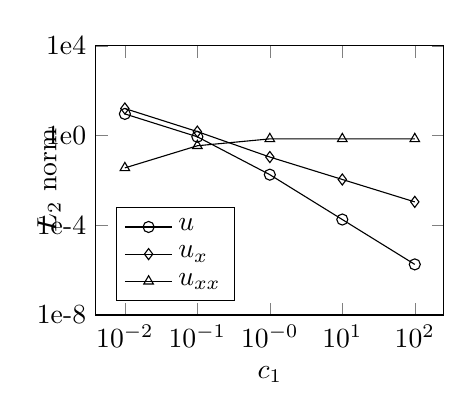
\begin{tikzpicture} 
\begin{axis}
[
    ymode=log,
    ymin=1e-8,
    ymax=1e4,
    ytick={1e-8, 1e-4, 1e0, 1e4},
    yticklabels={1e-8, 1e-4, 1e0, 1e4},
    legend style={at={(0.4,0.4)},nodes={scale=1}},
    legend cell align={left},
    height=5cm,
    width=6cm,
    xlabel={$c_1$},
    xlabel style={below},      
    ylabel={$L_2$ norm},
    ylabel style={below},    
    xtick=data,
    xticklabels={$10^{-2}$, $10^{-1}$, $10^{-0}$, $10^{1}$, $10^{2}$}    
]
\addplot[mark=o] coordinates {(0,9.2e0) (1,8.8e-1) (2,1.8e-2) (3,1.8e-4) (4,1.8e-6)}; 
\addplot[mark=diamond] coordinates {(0,1.6e1) (1,1.5e0) (2,1.1e-1) (3,1.1e-2) (4,1.1e-3)}; 
\addplot[mark=triangle] coordinates {(0,3.6e-2) (1,3.5e-1) (2,7.1e-1) (3,7.1e-1) (4,7.1e-1)}; 
\legend{$u$,$u_x$,$u_{xx}$};
\end{axis}
\end{tikzpicture}
}
\caption{Case 1}
\label{L2_norm_case_1}
\end{subfigure}
\hspace{0.15cm}
\begin{subfigure}[b]{0.3\textwidth}
\scalebox{0.9}{
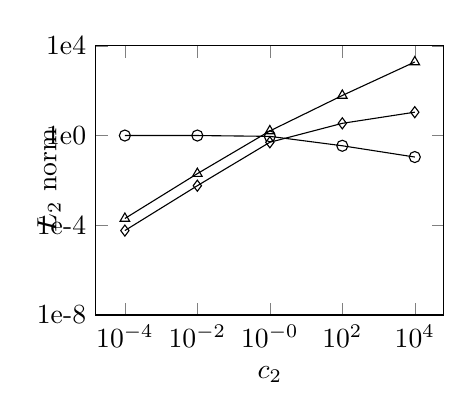
\begin{tikzpicture} 
\begin{axis}
[
    ymode=log,
    ymin=1e-8,
    ymax=1e4,
    ytick={1e-8, 1e-4, 1e0, 1e4},
    yticklabels={1e-8, 1e-4, 1e0, 1e4},    
    height=5cm,
    width=6cm,
    xlabel={$c_2$},
    xlabel style={below},      
    ylabel={$L_2$ norm},
    ylabel style={below},    
    xtick=data,
    xticklabels={$10^{-4}$, $10^{-2}$, $10^{-0}$, $10^{2}$, $10^{4}$}    
]
\addplot[mark=o] coordinates {(0, 1e0) (1, 1e0) (2, 0.92) (3, 0.35) (4, 0.11)}; 
\addplot[mark=diamond] coordinates {(0, 5.8e-5) (1, 5.8e-3) (2, 5.0e-1) (3, 3.5) (4, 11)}; 
\addplot[mark=triangle] coordinates {(0, 2.0e-4) (1, 2.0e-2) (2, 1.6) (3, 61) (4, 1.9e3)}; 
\end{axis}
\end{tikzpicture}
}
\caption{Case 2}
\label{L2_norm_case_2}
\end{subfigure}
\hspace{0.15cm}
\begin{subfigure}[b]{0.3\textwidth}
\scalebox{0.9}{
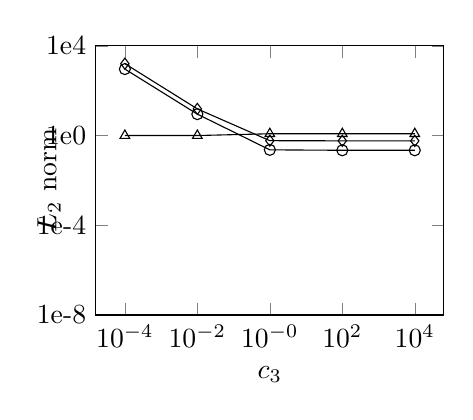
\begin{tikzpicture} 
\begin{axis}
[
    ymode=log,
    ymin=1e-8,
    ymax=1e4,
    ytick={1e-8, 1e-4, 1e0, 1e4},
    yticklabels={1e-8, 1e-4, 1e0, 1e4},    
    height=5cm,
    width=6cm,
    xlabel={$c_3$},
    xlabel style={below},      
    ylabel={$L_2$ norm},
    ylabel style={below},    
    xtick=data,
    xticklabels={$10^{-4}$, $10^{-2}$, $10^{-0}$, $10^{2}$, $10^{4}$}    
]
\addplot[mark=o] coordinates {(0, 920) (1, 9) (2, 0.23) (3, 0.22) (4, 0.22)}; 
\addplot[mark=diamond] coordinates {(0, 1.6e3) (1, 15.4) (2, 0.59) (3, 0.58) (4, 0.58)}; 
\addplot[mark=triangle] coordinates {(0, 1.0) (1, 1.0) (2, 1.2) (3, 1.2) (4, 1.2)}; 
\end{axis}
\end{tikzpicture}
}
\caption{Case 3}
\label{L2_norm_case_3}
\end{subfigure}

\hspace{2.5cm}
\begin{subfigure}[b]{0.3\textwidth}
\scalebox{0.9}{
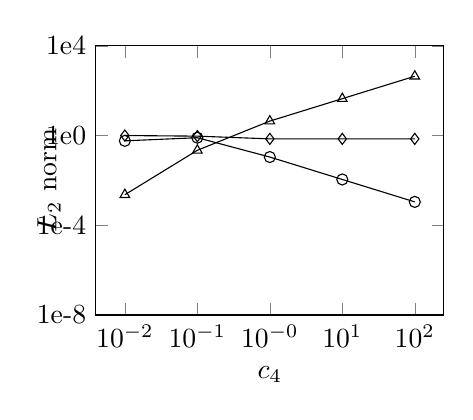
\begin{tikzpicture} 
\begin{axis}
[
    ymode=log,
    ymin=1e-8,
    ymax=1e4,
    ytick={1e-8, 1e-4, 1e0, 1e4},
    yticklabels={1e-8, 1e-4, 1e0, 1e4},    
    height=5cm,
    width=6cm,
    xlabel={$c_4$},
    xlabel style={below},      
    ylabel={$L_2$ norm},
    ylabel style={below},    
    xtick=data,
    xticklabels={$10^{-2}$, $10^{-1}$, $10^{-0}$, $10^{1}$, $10^{2}$}    
]
\addplot[mark=o] coordinates {(0, 0.58) (1, 0.8) (2, 1.1e-1) (3, 1.1e-2) (4, 1.1e-3)}; 
\addplot[mark=diamond] coordinates {(0, 1.0) (1, 0.94) (2, 0.71) (3, 0.71) (4, 0.71)}; 
\addplot[mark=triangle] coordinates {(0, 2.3e-3) (1, 0.22) (2, 4.4) (3, 4.4e1) (4, 4.4e2)}; 
\end{axis}
\end{tikzpicture}
}
\caption{Case 4}
\label{L2_norm_case_4}
\end{subfigure}
\hspace{0.15cm}
\begin{subfigure}[b]{0.3\textwidth}
\scalebox{0.9}{
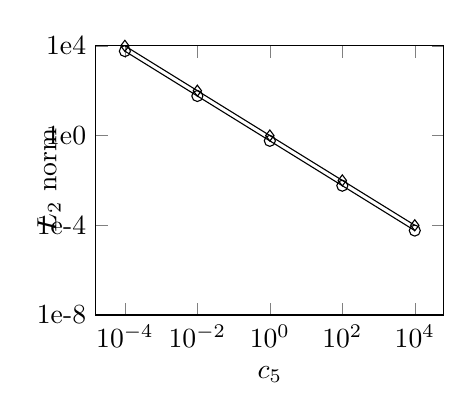
\begin{tikzpicture} 
\begin{axis}
[
    ymode=log,
    ymin=1e-8,
    ymax=1e4,
    ytick={1e-8, 1e-4, 1e0, 1e4},
    yticklabels={1e-8, 1e-4, 1e0, 1e4},    
    height=5cm,
    width=6cm,
    xlabel={$c_5$},
    xlabel style={below},      
    ylabel={$L_2$ norm},
    ylabel style={below},    
    xtick=data,
    xticklabels={$10^{-4}$, $10^{-2}$, $10^{0}$, $10^{2}$, $10^{4}$} 
]
\addplot[mark=o] coordinates {(0, 5800) (1, 58) (2, 0.58) (3, 5.8e-3) (4, 5.8e-5)}; 
\addplot[mark=diamond] coordinates {(0, 1e4) (1, 1e2) (2, 1) (3, 1e-2) (4, 1e-4)}; 
\addplot[mark=triangle] coordinates {(0, 0.0) (1, 0.0) (2, 0.0) (3, 0.0) (4, 0.0)}; 
\end{axis}
\end{tikzpicture}
}
\caption{Case 5}
\label{L2_norm_case_5}
\end{subfigure}
\caption{$L_2$ norms of $u$, $u_{x}$ and $u_{xx}$ for different cases.}
\label{L2_norms_cases_1_to_5}
\end{figure}

\newpage

\subsection{Absolute errors}

\subsubsection{The standard FEM}

% \newpage

\paragraph{Case 1}
For Case 1, using the standard FEM without scaling the right-hand side and scheme S, the absolute errors are shown in Figs. \ref{py_L2_Pois1_SM_scaling_no}--\ref{py_L2_Pois1_SM_scaling_S}.

\begin{figure}[!ht]
    \begin{subfigure}{5.5cm}
        \includegraphics[width=1.0\linewidth]{py_L2_Pois1_SM_scaling_no_solu.pdf}
        \caption{Solution}
        \label{py_L2_Pois1_SM_scaling_no_solu}
    \end{subfigure}
    \hspace{-0.2cm}
    \begin{subfigure}{5.5cm}
        \includegraphics[width=1.0\linewidth]{py_L2_Pois1_SM_scaling_no_grad.pdf}
        \caption{First derivative}
        \label{py_L2_Pois1_SM_scaling_no_grad}
    \end{subfigure}
    \hspace{-0.2cm}
    \begin{subfigure}{5.5cm}
        \includegraphics[width=1.0\linewidth]{py_L2_Pois1_SM_scaling_no_2ndd.pdf}
        \caption{Second derivative}
        \label{py_L2_Pois1_SM_scaling_no_2ndd}
    \end{subfigure}
\caption{Absolute errors for different $c_1$ using the standard FEM without scaling the right-hand side.}   
\label{py_L2_Pois1_SM_scaling_no}
\end{figure}

\begin{figure}[!ht]
    \begin{subfigure}{5.5cm}
        \includegraphics[width=1.0\linewidth]{py_L2_Pois1_SM_scaling_S_solu.pdf}
        \caption{Solution}
        \label{py_L2_Pois1_SM_scaling_S_solu}
    \end{subfigure}
    \hspace{-0.2cm}
    \begin{subfigure}{5.5cm}
        \includegraphics[width=1.0\linewidth]{py_L2_Pois1_SM_scaling_S_grad.pdf}
        \caption{First derivative}
        \label{py_L2_Pois1_SM_scaling_S_grad}
    \end{subfigure}
    \hspace{-0.2cm}
    \begin{subfigure}{5.5cm}
        \includegraphics[width=1.0\linewidth]{py_L2_Pois1_SM_scaling_S_2ndd.pdf}
        \caption{Second derivative}
        \label{py_L2_Pois1_SM_scaling_S_2ndd}
    \end{subfigure}
\caption{Absolute errors for different $c_1$ using the standard FEM with scheme $S$.}    
\label{py_L2_Pois1_SM_scaling_S}
\end{figure}

\newpage

\paragraph{Case 2}
For Case 2, using the standard FEM without scaling the right-hand side and scheme S, the absolute errors are shown in Figs. \ref{py_L2_Pois2_SM_scaling_no}--\ref{py_L2_Pois2_SM_scaling_S}.

\begin{figure}[!ht]
    \begin{subfigure}{5.5cm}
        \includegraphics[width=1.0\linewidth]{py_L2_Pois2_SM_scaling_no_solu.pdf}
        \caption{Solution}
        \label{py_L2_Pois2_SM_scaling_no_solu}
    \end{subfigure}
    \hspace{-0.2cm}
    \begin{subfigure}{5.5cm}
        \includegraphics[width=1.0\linewidth]{py_L2_Pois2_SM_scaling_no_grad.pdf}
        \caption{First derivative}
        \label{py_L2_Pois2_SM_scaling_no_grad}
    \end{subfigure}
    \hspace{-0.2cm}
    \begin{subfigure}{5.5cm}
        \includegraphics[width=1.0\linewidth]{py_L2_Pois2_SM_scaling_no_2ndd.pdf}
        \caption{Second derivative}
        \label{py_L2_Pois2_SM_scaling_no_2ndd}
    \end{subfigure}
\caption{Absolute errors for Case 2 using the standard FEM without scaling the right-hand side.}
\label{py_L2_Pois2_SM_scaling_no}
\end{figure}

\begin{figure}[!ht]
    \begin{subfigure}{5.5cm}
        \includegraphics[width=1.0\linewidth]{py_L2_Pois2_SM_scaling_S_solu.pdf}
        \caption{Solution}
        \label{py_L2_Pois2_SM_scaling_S_solu}
    \end{subfigure}
    \hspace{-0.2cm}
    \begin{subfigure}{5.5cm}
        \includegraphics[width=1.0\linewidth]{py_L2_Pois2_SM_scaling_S_grad.pdf}
        \caption{First derivative}
        \label{py_L2_Pois2_SM_scaling_S_grad}
    \end{subfigure}
    \hspace{-0.2cm}
    \begin{subfigure}{5.5cm}
        \includegraphics[width=1.0\linewidth]{py_L2_Pois2_SM_scaling_S_2ndd.pdf}
        \caption{Second derivative}
        \label{py_L2_Pois2_SM_scaling_S_2ndd}
    \end{subfigure}
\caption{Absolute errors for Case 2 using scheme $S$.}
\label{py_L2_Pois2_SM_scaling_S}
\end{figure}

% \newpage
\paragraph{Case 3}
For Case 3, using the standard FEM without scaling the right-hand side and scheme S, the absolute errors are shown in Figs. \ref{py_L2_Pois3_SM_scaling_no}--\ref{py_L2_Pois3_SM_scaling_S}.

\begin{figure}[!ht]
    \begin{subfigure}{5.5cm}
        \includegraphics[width=1.0\linewidth]{py_L2_Pois3_SM_scaling_no_solu.pdf}
        \caption{Solution}
        \label{py_L2_Pois3_SM_scaling_no_solu}
    \end{subfigure}
    \hspace{-0.2cm}
    \begin{subfigure}{5.5cm}
        \includegraphics[width=1.0\linewidth]{py_L2_Pois3_SM_scaling_no_grad.pdf}
        \caption{First derivative}
        \label{py_L2_Pois3_SM_scaling_no_grad}
    \end{subfigure}
    \hspace{-0.2cm}
    \begin{subfigure}{5.5cm}
        \includegraphics[width=1.0\linewidth]{py_L2_Pois3_SM_scaling_no_2ndd.pdf}
        \caption{Second derivative}
        \label{py_L2_Pois3_SM_scaling_no_2ndd}
    \end{subfigure}
\caption{Absolute errors for Case 3 using the standard FEM without scaling the right-hand side.}
\label{py_L2_Pois3_SM_scaling_no}
\end{figure}

\begin{figure}[!ht]
    \begin{subfigure}{5.5cm}
        \includegraphics[width=1.0\linewidth]{py_L2_Pois3_SM_scaling_S_solu.pdf}
        \caption{Solution}
        \label{py_L2_Pois3_SM_scaling_S_solu}
    \end{subfigure}
    \hspace{-0.2cm}
    \begin{subfigure}{5.5cm}
        \includegraphics[width=1.0\linewidth]{py_L2_Pois3_SM_scaling_S_grad.pdf}
        \caption{First derivative}
        \label{py_L2_Pois3_SM_scaling_S_grad}
    \end{subfigure}
    \hspace{-0.2cm}
    \begin{subfigure}{5.5cm}
        \includegraphics[width=1.0\linewidth]{py_L2_Pois3_SM_scaling_S_2ndd.pdf}
        \caption{Second derivative}
        \label{py_L2_Pois3_SM_scaling_S_2ndd}
    \end{subfigure}
\caption{Absolute errors of Case 3 using scheme $S$.}
\label{py_L2_Pois3_SM_scaling_S}
\end{figure}

\newpage
\paragraph{Case 4}
For Case 4, using the standard FEM without scaling the right-hand side and scheme S, the absolute errors are shown in Figs. \ref{py_L2_Pois4_SM_scaling_no}--\ref{py_L2_Pois4_SM_scaling_S}.

\begin{figure}[!ht]
    \begin{subfigure}{5.5cm}
        \includegraphics[width=1.0\linewidth]{py_L2_Pois4_SM_scaling_no_solu.pdf}
        \caption{Solution}
        \label{py_L2_Pois4_SM_scaling_no_solu}
    \end{subfigure}
    \hspace{-0.2cm}
    \begin{subfigure}{5.5cm}
        \includegraphics[width=1.0\linewidth]{py_L2_Pois4_SM_scaling_no_grad.pdf}
        \caption{First derivative}
        \label{py_L2_Pois4_SM_scaling_no_grad}
    \end{subfigure}
    \hspace{-0.2cm}
    \begin{subfigure}{5.5cm}
        \includegraphics[width=1.0\linewidth]{py_L2_Pois4_SM_scaling_no_2ndd.pdf}
        \caption{Second derivative}
        \label{py_L2_Pois4_SM_scaling_no_2ndd}
    \end{subfigure}
\caption{Absolute errors for Case 4 using the standard FEM without scaling the right-hand side.}
\label{py_L2_Pois4_SM_scaling_no}
\end{figure}

\begin{figure}[!ht]
    \begin{subfigure}{5.5cm}
        \includegraphics[width=1.0\linewidth]{py_L2_Pois4_SM_scaling_S_solu.pdf}
        \caption{Solution}
        \label{py_L2_Pois4_SM_scaling_S_solu}
    \end{subfigure}
    \hspace{-0.2cm}
    \begin{subfigure}{5.5cm}
        \includegraphics[width=1.0\linewidth]{py_L2_Pois4_SM_scaling_S_grad.pdf}
        \caption{First derivative}
        \label{py_L2_Pois4_SM_scaling_S_grad}
    \end{subfigure}
    \hspace{-0.2cm}
    \begin{subfigure}{5.5cm}
        \includegraphics[width=1.0\linewidth]{py_L2_Pois4_SM_scaling_S_2ndd.pdf}
        \caption{Second derivative}
        \label{py_L2_Pois4_SM_scaling_S_2ndd}
    \end{subfigure}
\caption{Absolute errors of Case 4 using scheme $S$.}
\label{py_L2_Pois4_SM_scaling_S}
\end{figure}

\newpage
\paragraph{Case 5}
For Case 5, using the standard FEM without scaling the right-hand side and scheme S, the absolute errors are shown in Figs. \ref{py_L2_Pois5_SM_scaling_no}--\ref{py_L2_Pois5_SM_scaling_S}.

\begin{figure}[!ht]
    \begin{subfigure}{5.5cm}
        \includegraphics[width=1.0\linewidth]{py_L2_Pois5_SM_scaling_no_solu.pdf}
        \caption{Solution}
        \label{py_L2_Pois5_SM_scaling_no_solu}
    \end{subfigure}
    \hspace{-0.2cm}
    \begin{subfigure}{5.5cm}
        \includegraphics[width=1.0\linewidth]{py_L2_Pois5_SM_scaling_no_grad.pdf}
        \caption{First derivative}
        \label{py_L2_Pois5_SM_scaling_no_grad}
    \end{subfigure}
    \hspace{-0.2cm}
    \begin{subfigure}{5.5cm}
        \includegraphics[width=1.0\linewidth]{py_L2_Pois5_SM_scaling_no_2ndd.pdf}
        \caption{Second derivative}
        \label{py_L2_Pois5_SM_scaling_no_2ndd}
    \end{subfigure}
\caption{Absolute errors for Case 5 using the standard FEM without scaling the right-hand side.}
\label{py_L2_Pois5_SM_scaling_no}
\end{figure}

\begin{figure}[!ht]
    \begin{subfigure}{5.5cm}
        \includegraphics[width=1.0\linewidth]{py_L2_Pois5_SM_scaling_S_solu.pdf}
        \caption{Solution}
        \label{py_L2_Pois5_SM_scaling_S_solu}
    \end{subfigure}
    \hspace{-0.2cm}
    \begin{subfigure}{5.5cm}
        \includegraphics[width=1.0\linewidth]{py_L2_Pois5_SM_scaling_S_grad.pdf}
        \caption{First derivative}
        \label{py_L2_Pois5_SM_scaling_S_grad}
    \end{subfigure}
    \hspace{-0.2cm}
    \begin{subfigure}{5.5cm}
        \includegraphics[width=1.0\linewidth]{py_L2_Pois5_SM_scaling_S_2ndd.pdf}
        \caption{Second derivative}
        \label{py_L2_Pois5_SM_scaling_S_2ndd}
    \end{subfigure}
\caption{Absolute errors of Case 5 using scheme $S$.}
\label{py_L2_Pois5_SM_scaling_S}
\end{figure}

\clearpage

\subsubsection{The mixed FEM}

\paragraph{Case 1}
For Case 1, using the mixed FEM without scaling the right-hand side and schemes ${\rm M}_1$ and ${\rm M}_2$, the absolute errors are shown in Figs. \ref{py_L2_Pois1_MM_scaling_no}--\ref{py_L2_Pois1_MM_scaling_M2}.


\begin{figure}[!ht]
    \begin{subfigure}{5.5cm}
        \includegraphics[width=1.0\linewidth]{py_L2_Pois1_MM_scaling_no_solu.pdf}
        \caption{Solution}
        \label{py_L2_Pois1_MM_scaling_no_solu}
    \end{subfigure}
    \hspace{-0.2cm}
    \begin{subfigure}{5.5cm}
        \includegraphics[width=1.0\linewidth]{py_L2_Pois1_MM_scaling_no_grad.pdf}
        \caption{First derivative}
        \label{py_L2_Pois1_MM_scaling_no_grad}
    \end{subfigure}
    \hspace{-0.2cm}
    \begin{subfigure}{5.5cm}
        \includegraphics[width=1.0\linewidth]{py_L2_Pois1_MM_scaling_no_2ndd.pdf}
        \caption{Second derivative}
        \label{py_L2_Pois1_MM_scaling_no_2ndd}
    \end{subfigure}
\caption{Absolute errors for different $c_1$ using the mixed FEM without scaling the right-hand side.}    
\label{py_L2_Pois1_MM_scaling_no}
\end{figure}

\vspace{0.0cm}
\begin{figure}[!ht]
    \begin{subfigure}{5.5cm}
        \includegraphics[width=1.0\linewidth]{py_L2_Pois1_MM_scaling_M1_solu.pdf}
        \caption{Solution}
        \label{py_L2_Pois1_MM_scaling_M1_solu}
    \end{subfigure}
    \hspace{-0.2cm}
    \begin{subfigure}{5.5cm}
        \includegraphics[width=1.0\linewidth]{py_L2_Pois1_MM_scaling_M1_grad.pdf}
        \caption{First derivative}
        \label{py_L2_Pois1_MM_scaling_M1_grad}
    \end{subfigure}
    \hspace{-0.2cm}
    \begin{subfigure}{5.5cm}
        \includegraphics[width=1.0\linewidth]{py_L2_Pois1_MM_scaling_M1_2ndd.pdf}
        \caption{Second derivative}
        \label{py_L2_Pois1_MM_scaling_M1_2ndd}
    \end{subfigure}
\caption{Absolute errors for different $c_1$ using the mixed FEM with scheme $M_1$.}    
\label{py_L2_Pois1_MM_scaling_M1}
\end{figure}

\begin{figure}[!ht]
    \begin{subfigure}{5.5cm}
        \includegraphics[width=1.0\linewidth]{py_L2_Pois1_MM_scaling_M2_solu.pdf}
        \caption{Solution}
        \label{py_L2_Pois1_MM_scaling_M2_solu}
    \end{subfigure}
    \hspace{-0.2cm}
    \begin{subfigure}{5.5cm}
        \includegraphics[width=1.0\linewidth]{py_L2_Pois1_MM_scaling_M2_grad.pdf}
        \caption{First derivative}
        \label{py_L2_Pois1_MM_scaling_M2_grad}
    \end{subfigure}
    \hspace{-0.2cm}
    \begin{subfigure}{5.5cm}
        \includegraphics[width=1.0\linewidth]{py_L2_Pois1_MM_scaling_M2_2ndd.pdf}
        \caption{Second derivative}
        \label{py_L2_Pois1_MM_scaling_M2_2ndd}
    \end{subfigure}
\caption{Absolute errors for different $c_1$ using the mixed FEM with scheme $M_2$.}
\label{py_L2_Pois1_MM_scaling_M2}
\end{figure}


\paragraph{Case 2}
For Case 2, using the mixed FEM without scaling the right-hand side and schemes ${\rm M}_1$ and ${\rm M}_2$, the absolute errors are shown in Figs. \ref{py_L2_Pois2_MM_scaling_no}--\ref{py_L2_Pois2_MM_scaling_M2}.

\begin{figure}[!ht]
    \begin{subfigure}{5.5cm}
        \includegraphics[width=1.0\linewidth]{py_L2_Pois2_MM_scaling_no_solu.pdf}
        \caption{Solution}
        \label{py_L2_Pois2_MM_scaling_no_solu}
    \end{subfigure}
    \hspace{-0.2cm}
    \begin{subfigure}{5.5cm}
        \includegraphics[width=1.0\linewidth]{py_L2_Pois2_MM_scaling_no_grad.pdf}
        \caption{First derivative}
        \label{py_L2_Pois2_MM_scaling_no_grad}
    \end{subfigure}
    \hspace{-0.2cm}
    \begin{subfigure}{5.5cm}
        \includegraphics[width=1.0\linewidth]{py_L2_Pois2_MM_scaling_no_2ndd.pdf}
        \caption{Second derivative}
        \label{py_L2_Pois2_MM_scaling_no_2ndd}
    \end{subfigure}
\caption{Absolute errors for Case 2 using the mixed FEM without scaling the right-hand side.}
\label{py_L2_Pois2_MM_scaling_no}
\end{figure}

\begin{figure}[!ht]
    \begin{subfigure}{5.5cm}
        \includegraphics[width=1.0\linewidth]{py_L2_Pois2_MM_scaling_M1_solu.pdf}
        \caption{Solution}
        \label{py_L2_Pois2_MM_scaling_M1_solu}
    \end{subfigure}
    \hspace{-0.2cm}
    \begin{subfigure}{5.5cm}
        \includegraphics[width=1.0\linewidth]{py_L2_Pois2_MM_scaling_M1_grad.pdf}
        \caption{First derivative}
        \label{py_L2_Pois2_MM_scaling_M1_grad}
    \end{subfigure}
    \hspace{-0.2cm}
    \begin{subfigure}{5.5cm}
        \includegraphics[width=1.0\linewidth]{py_L2_Pois2_MM_scaling_M1_2ndd.pdf}
        \caption{Second derivative}
        \label{py_L2_Pois2_MM_scaling_M1_2ndd}
    \end{subfigure}
\caption{Absolute errors for Case 2 using scheme $M_1$.}
\label{py_L2_Pois2_MM_scaling_M1}
\end{figure}

\begin{figure}[!ht]
    \begin{subfigure}{5.5cm}
        \includegraphics[width=1.0\linewidth]{py_L2_Pois2_MM_scaling_M2_solu.pdf}
        \caption{Solution}
        \label{py_L2_Pois2_MM_scaling_M2_solu}
    \end{subfigure}
    \hspace{-0.2cm}
    \begin{subfigure}{5.5cm}
        \includegraphics[width=1.0\linewidth]{py_L2_Pois2_MM_scaling_M2_grad.pdf}
        \caption{First derivative}
        \label{py_L2_Pois2_MM_scaling_M2_grad}
    \end{subfigure}
    \hspace{-0.2cm}
    \begin{subfigure}{5.5cm}
        \includegraphics[width=1.0\linewidth]{py_L2_Pois2_MM_scaling_M2_2ndd.pdf}
        \caption{Second derivative}
        \label{py_L2_Pois2_MM_scaling_M2_2ndd}
    \end{subfigure}
\caption{Absolute errors for Case 2 using scheme $M_2$.}
\label{py_L2_Pois2_MM_scaling_M2}
\end{figure}

\newpage
\paragraph{Case 3}
For Case 3, using the mixed FEM without scaling the right-hand side and schemes ${\rm M}_1$ and ${\rm M}_2$, the absolute errors are shown in Figs. \ref{py_L2_Pois3_MM_scaling_no}--\ref{py_L2_Pois3_MM_scaling_M2}.

\begin{figure}[!ht]
    \begin{subfigure}{5.5cm}
        \includegraphics[width=1.0\linewidth]{py_L2_Pois3_MM_scaling_no_solu.pdf}
        \caption{Solution}
        \label{py_L2_Pois3_MM_scaling_no_solu}
    \end{subfigure}
    \hspace{-0.2cm}
    \begin{subfigure}{5.5cm}
        \includegraphics[width=1.0\linewidth]{py_L2_Pois3_MM_scaling_no_grad.pdf}
        \caption{First derivative}
        \label{py_L2_Pois3_MM_scaling_no_grad}
    \end{subfigure}
    \hspace{-0.2cm}
    \begin{subfigure}{5.5cm}
        \includegraphics[width=1.0\linewidth]{py_L2_Pois3_MM_scaling_no_2ndd.pdf}
        \caption{Second derivative}
        \label{py_L2_Pois3_MM_scaling_no_2ndd}
    \end{subfigure}
\caption{Absolute errors for Case 3 using the mixed FEM without scaling the right-hand side.}
\label{py_L2_Pois3_MM_scaling_no}
\end{figure}

\begin{figure}[!ht]
    \begin{subfigure}{5.5cm}
        \includegraphics[width=1.0\linewidth]{py_L2_Pois3_MM_scaling_M1_solu.pdf}
        \caption{Solution}
        \label{py_L2_Pois3_MM_scaling_M1_solu}
    \end{subfigure}
    \hspace{-0.2cm}
    \begin{subfigure}{5.5cm}
        \includegraphics[width=1.0\linewidth]{py_L2_Pois3_MM_scaling_M1_grad.pdf}
        \caption{First derivative}
        \label{py_L2_Pois3_MM_scaling_M1_grad}
    \end{subfigure}
    \hspace{-0.2cm}
    \begin{subfigure}{5.5cm}
        \includegraphics[width=1.0\linewidth]{py_L2_Pois3_MM_scaling_M1_2ndd.pdf}
        \caption{Second derivative}
        \label{py_L2_Pois3_MM_scaling_M1_2ndd}
    \end{subfigure}
\caption{Absolute errors for Case 3 using scheme $M_1$.}
\label{py_L2_Pois3_MM_scaling_M1}
\end{figure}

\begin{figure}[!ht]
    \begin{subfigure}{5.5cm}
        \includegraphics[width=1.0\linewidth]{py_L2_Pois3_MM_scaling_M2_solu.pdf}
        \caption{Solution}
        \label{py_L2_Pois3_MM_scaling_M2_solu}
    \end{subfigure}
    \hspace{-0.2cm}
    \begin{subfigure}{5.5cm}
        \includegraphics[width=1.0\linewidth]{py_L2_Pois3_MM_scaling_M2_grad.pdf}
        \caption{First derivative}
        \label{py_L2_Pois3_MM_scaling_M2_grad}
    \end{subfigure}
    \hspace{-0.2cm}
    \begin{subfigure}{5.5cm}
        \includegraphics[width=1.0\linewidth]{py_L2_Pois3_MM_scaling_M2_2ndd.pdf}
        \caption{Second derivative}
        \label{py_L2_Pois3_MM_scaling_M2_2ndd}
    \end{subfigure}
\caption{Absolute errors for Case 3 using scheme $M_2$.}
\label{py_L2_Pois3_MM_scaling_M2}
\end{figure}

\newpage
\paragraph{Case 4}
For Case 4, using the mixed FEM without scaling the right-hand side and schemes ${\rm M}_1$ and ${\rm M}_2$, the absolute errors are shown in Figs. \ref{py_L2_Pois4_MM_scaling_no}--\ref{py_L2_Pois4_MM_scaling_M2}.

\begin{figure}[!ht]
    \begin{subfigure}{5.5cm}
        \includegraphics[width=1.0\linewidth]{py_L2_Pois4_MM_scaling_no_solu.pdf}
        \caption{Solution}
        \label{py_L2_Pois4_MM_scaling_no_solu}
    \end{subfigure}
    \hspace{-0.2cm}
    \begin{subfigure}{5.5cm}
        \includegraphics[width=1.0\linewidth]{py_L2_Pois4_MM_scaling_no_grad.pdf}
        \caption{First derivative}
        \label{py_L2_Pois4_MM_scaling_no_grad}
    \end{subfigure}
    \hspace{-0.2cm}
    \begin{subfigure}{5.5cm}
        \includegraphics[width=1.0\linewidth]{py_L2_Pois4_MM_scaling_no_2ndd.pdf}
        \caption{Second derivative}
        \label{py_L2_Pois4_MM_scaling_no_2ndd}
    \end{subfigure}
\caption{Absolute errors for Case 4 using the mixed FEM without scaling the right-hand side.}
\label{py_L2_Pois4_MM_scaling_no}
\end{figure}

\begin{figure}[!ht]
    \begin{subfigure}{5.5cm}
        \includegraphics[width=1.0\linewidth]{py_L2_Pois4_MM_scaling_M1_solu.pdf}
        \caption{Solution}
        \label{py_L2_Pois4_MM_scaling_M1_solu}
    \end{subfigure}
    \hspace{-0.2cm}
    \begin{subfigure}{5.5cm}
        \includegraphics[width=1.0\linewidth]{py_L2_Pois4_MM_scaling_M1_grad.pdf}
        \caption{First derivative}
        \label{py_L2_Pois4_MM_scaling_M1_grad}
    \end{subfigure}
    \hspace{-0.2cm}
    \begin{subfigure}{5.5cm}
        \includegraphics[width=1.0\linewidth]{py_L2_Pois4_MM_scaling_M1_2ndd.pdf}
        \caption{Second derivative}
        \label{py_L2_Pois4_MM_scaling_M1_2ndd}
    \end{subfigure}
\caption{Absolute errors for Case 4 using scheme $M_1$.}
\label{py_L2_Pois4_MM_scaling_M1}
\end{figure}

\begin{figure}[!ht]
    \begin{subfigure}{5.5cm}
        \includegraphics[width=1.0\linewidth]{py_L2_Pois4_MM_scaling_M2_solu.pdf}
        \caption{Solution}
        \label{py_L2_Pois4_MM_scaling_M2_solu}
    \end{subfigure}
    \hspace{-0.2cm}
    \begin{subfigure}{5.5cm}
        \includegraphics[width=1.0\linewidth]{py_L2_Pois4_MM_scaling_M2_grad.pdf}
        \caption{First derivative}
        \label{py_L2_Pois4_MM_scaling_M2_grad}
    \end{subfigure}
    \hspace{-0.2cm}
    \begin{subfigure}{5.5cm}
        \includegraphics[width=1.0\linewidth]{py_L2_Pois4_MM_scaling_M2_2ndd.pdf}
        \caption{Second derivative}
        \label{py_L2_Pois4_MM_scaling_M2_2ndd}
    \end{subfigure}
\caption{Absolute errors for Case 4 using scheme $M_2$.}
\label{py_L2_Pois4_MM_scaling_M2}
\end{figure}
% 

\newpage
\paragraph{Case 5}
For Case 5, using the mixed FEM without scaling the right-hand side and schemes ${\rm M}_1$, the absolute errors are shown in Figs. \ref{py_L2_Pois5_MM_scaling_no}--\ref{py_L2_Pois5_MM_scaling_M1}.

\begin{figure}[!ht]
    \begin{subfigure}{5.5cm}
        \includegraphics[width=1.0\linewidth]{py_L2_Pois5_MM_scaling_no_solu.pdf}
        \caption{Solution}
        \label{py_L2_Pois5_MM_scaling_no_solu}
    \end{subfigure}
    \hspace{-0.2cm}
    \begin{subfigure}{5.5cm}
        \includegraphics[width=1.0\linewidth]{py_L2_Pois5_MM_scaling_no_grad.pdf}
        \caption{First derivative}
        \label{py_L2_Pois5_MM_scaling_no_grad}
    \end{subfigure}
    \hspace{-0.2cm}
    \begin{subfigure}{5.5cm}
        \includegraphics[width=1.0\linewidth]{py_L2_Pois5_MM_scaling_no_2ndd.pdf}
        \caption{Second derivative}
        \label{py_L2_Pois5_MM_scaling_no_2ndd}
    \end{subfigure}
\caption{Absolute errors for Case 5 using the mixed FEM without scaling the right-hand side.}
\label{py_L2_Pois5_MM_scaling_no}
\end{figure}

\begin{figure}[!ht]
    \begin{subfigure}{5.5cm}
        \includegraphics[width=1.0\linewidth]{py_L2_Pois5_MM_scaling_M1_solu.pdf}
        \caption{Solution}
        \label{py_L2_Pois5_MM_scaling_M1_solu}
    \end{subfigure}
    \hspace{-0.2cm}
    \begin{subfigure}{5.5cm}
        \includegraphics[width=1.0\linewidth]{py_L2_Pois5_MM_scaling_M1_grad.pdf}
        \caption{First derivative}
        \label{py_L2_Pois5_MM_scaling_M1_grad}
    \end{subfigure}
    \hspace{-0.2cm}
    \begin{subfigure}{5.5cm}
        \includegraphics[width=1.0\linewidth]{py_L2_Pois5_MM_scaling_M1_2ndd.pdf}
        \caption{Second derivative}
        \label{py_L2_Pois5_MM_scaling_M1_2ndd}
    \end{subfigure}
\caption{Absolute errors for Case 5 using scheme $M_1$.}
\label{py_L2_Pois5_MM_scaling_M1}
\end{figure}

\begin{figure}[!ht]
    \begin{subfigure}{5.5cm}
        \includegraphics[width=1.0\linewidth]{py_L2_Pois5_MM_scaling_M2_solu.pdf}
        \caption{Solution}
        \label{py_L2_Pois5_MM_scaling_M2_solu}
    \end{subfigure}
    \hspace{-0.2cm}
    \begin{subfigure}{5.5cm}
        \includegraphics[width=1.0\linewidth]{py_L2_Pois5_MM_scaling_M2_grad.pdf}
        \caption{First derivative}
        \label{py_L2_Pois5_MM_scaling_M2_grad}
    \end{subfigure}
    \hspace{-0.2cm}
    \begin{subfigure}{5.5cm}
        \includegraphics[width=1.0\linewidth]{py_L2_Pois5_MM_scaling_M2_2ndd.pdf}
        \caption{Second derivative}
        \label{py_L2_Pois5_MM_scaling_M2_2ndd}
    \end{subfigure}
\caption{Absolute errors for Case 5 using scheme $M_2$.}
\label{py_L2_Pois5_MM_scaling_M2}
\end{figure}

% \newpage
% 
\bibliographystyle{unsrt}  
\bibliography{mybibfile}  %%% Remove comment to use the external .bib file (using bibtex).


\end{document}
